%% Преамбула TeX-файла
%% 1. Стиль и язык
\documentclass[utf8x, 12pt]{G7-32} % Стиль (по умолчанию будет 14pt)
\usepackage{cmap}
\usepackage{verbatim}
\usepackage[utf8x]{inputenc} % Включаем поддержку UTF8  
\usepackage[russian]{babel}



% Остальные стандартные настройки убраны в preamble.inc.tex.
\sloppy

% Настройки стиля ГОСТ 7-32
% Для начала определяем, хотим мы или нет, чтобы рисунки и таблицы нумеровались в пределах раздела, или нам нужна сквозная нумерация.
\EqInChapter % формулы будут нумероваться в пределах раздела
\TableInChapter % таблицы будут нумероваться в пределах раздела
\PicInChapter % рисунки будут нумероваться в пределах раздела

% Добавляем гипертекстовое оглавление в PDF
\usepackage[
bookmarks=true, colorlinks=true, unicode=true,
urlcolor=black,linkcolor=black, anchorcolor=black,
citecolor=black, menucolor=black, filecolor=black,
]{hyperref}

% Изменение начертания шрифта --- после чего выглядит таймсоподобно.
% apt-get install scalable-cyrfonts-tex

\IfFileExists{cyrtimes.sty}
    {
        \usepackage{cyrtimespatched}
    }
    {
        % А если Times нету, то будет CM...
    }

\usepackage{graphicx}   % Пакет для включения рисунков
\DeclareGraphicsExtensions{.jpg,.pdf,.png,.odg}
% С такими оно полями оно работает по-умолчанию:
% \RequirePackage[left=20mm,right=10mm,top=20mm,bottom=20mm,headsep=0pt]{geometry}
% Если вас тошнит от поля в 10мм --- увеличивайте до 20-ти, ну и про переплёт не забывайте:
\geometry{right=20mm}
\geometry{left=30mm}



% Произвольная нумерация списков.
\usepackage{enumerate}
\usepackage{enumitem}

\setcounter{tocdepth}{2} %Подробность оглавления
%4 это chapter, section, subsection, subsubsection и paragraph
%3 это chapter, section, subsection и subsubsection
%2 это chapter, section, и subsection
%1 это chapter и section
%0 это chapter.

\usepackage{epstopdf}
\begin{document}

\frontmatter % выключает нумерацию ВСЕГО; здесь начинаются ненумерованные главы: реферат, введение, глоссарий, сокращения и прочее.
\begin{center} 

\large НИУ "Высшая школа экономики"\\ 
\large Московский институт электроники и математики"\\[5.5cm] 

\huge Описание программы  \\[0.6cm] % название работы, затем отступ 0,6см
\large и её применения\\[3.7cm]


\end{center} 

\begin{flushright}
Юлдашев А. Х.  \\
\end{flushright}


\vfill 

\begin{center} 
\large Москва 2024
\end{center} 

\thispagestyle{empty}

\thispagestyle{empty}
\setcounter{page}{0}
\tableofcontents
\clearpage

\chapter{Введение}
\label{intro:0}
\begin{flushleft}

Для написания и тестирования программы были установлены:

\begin{itemize}
	\item[-] Заголовочные и исходные файлы ядра Linux версии 6.1;
	\item[-] libbpf пакет версии 1.4 (с оптимизацией llvm);
\end{itemize}
Настройки окружения:
\begin{itemize}
	\item[-] Операционная система Arch Linux;
	\item[-] Ядро версии 6.9.3;
	\item[-] gcc версии 14.1;
\end{itemize}


В дальнейшем понадобиться дампить объектные файлы для чтения их инструкций, для этого применяется:
\begin{verbatim}
	llvm-objdump-14 -d *.bpf.o
	или
	llvm-objdump -d *.bpf.o
\end{verbatim}

\ \\
Модуль (kernel security module) deny\_unshare применяется для контроля системного вызова unshare, при создании нового пространства.\\

\ \\
Для использования модуля необходимо:
\begin{itemize}
	\item[1.] Собрать все необходимые пакеты для компиляции BPF программ.
	\item[2.] Собрать исполняемый файл.
	\item[3.] запустить исполняемый файл:
	\begin{verbatim}
					./<file_name>
	\end{verbatim}
\end{itemize}


Для прекращения работы программы нужно послать сигнал SIGINT/INT (например, просто в терминале процесса нажать Ctrl+C).
\\ \

Для тестирования работоспособности программы применяются попытки создания нового пространства.
\end{flushleft}



\mainmatter

\chapter{Теория. Основы.}
\label{theory-base-0}
\begin{flushleft}
	
Данный документ не затрагивает развитие мысли вредоносности неконтролируемого создания пространств любым пользователем, поэтому ограничимся тем, что это приводит к большой проблеме безопасности для НОВЫХ пользователей подобных систем. Для примера применения приведу возможность "масштабирования" подобного пространства для того, что бы новые пользователи вносили свои данные в уже захваченную среду/систему. Так же, благодаря этому можно "выйти" из ограниченного окружения, что подробно описано в  \href{https://book.hacktricks.xyz/linux-hardening/privilege-escalation/docker-security/namespaces/user-namespace}{\textcolor{blue}{этой}} статье. \\

Начну с пояснения используемых инструментов:
\begin{itemize}
	\item[1.] Технология BPF (см. главу \underline{\nameref{theory-bpf-0}})
	\item[2.] Технология LSM (см. главу \underline{\nameref{theory-lsm-0}})
\end{itemize}
Для дальнейшего чтения стоит ознакомиться с соответствующими вышему главами.

Для работы этих двух инструментов была использована внутренняя возможность LSM и BPF, которые изначально позволяют удобно внедрять BPF инструкции к LSM хукам.

\end{flushleft}
\section{Теория. BPF.}
\label{theory-bpf-0}

\begin{flushleft}
	
\paragraph{Введение}

	Технология BPF (Berkeley Packet Filter) изначально была разработана для фильтрации пакетов в сетевых приложениях, таких как tcpdump. Однако со временем BPF значительно эволюционировал, особенно в контексте ядра Linux, превратившись в мощный механизм, используемый для различных целей, включая мониторинг производительности, сетевую безопасность и диагностику.
	
\paragraph{Исходная концепция}

\begin{itemize}
	\item[•] BPF был представлен в 1992 году как эффективный способ фильтрации пакетов в операционной системе BSD.
	\item[•] Исходный BPF включал в себя байт-код, который выполняется в виртуальной машине внутри ядра, что позволяло быстро и эффективно обрабатывать сетевые пакеты.
	\item[•] Изолированность среды выполнения BPF инструкций (байт-код, описанный выше).
\end{itemize}

\paragraph{eBPF: Расширенный BPF}

eBPF (extended BPF) — это значительно расширенная версия оригинального BPF:
\begin{itemize}
	\item[•] Введение в ядре Linux: eBPF был интегрирован в ядро Linux начиная с версии 3.15.
	\item[•] Расширение функциональности: eBPF позволяет выполнять произвольный код в ядре, что открывает возможности для различных типов мониторинга и обработки данных.
	\item[•] Поддержка новых типов карт eBPF (BPF maps), которые являются ключевым элементом для хранения и обмена данными между программами eBPF и пользовательским пространством.
	\item[•] Расширенная поддержка проб eBPF. Пробы (probes) eBPF используются для динамической вставки точек отслеживания в код ядра.
	\item[•] BPF Type Format (BTF) — это новый формат, позволяющий программам eBPF получать доступ к информации о типах данных в ядре Linux.
	\item[*] Остальные инновации нас интересовать будут меньше.
\end{itemize}


\newpage

\paragraph{Архитектура и компоненты eBPF}

\begin{itemize}
	\item[1.] Программы eBPF:
		\begin{itemize}
			\item[•] Написаны на высокоуровневом языке, таком как C, и затем компилируются в байт-код eBPF.
			\item[•] Загружаются в ядро через системные вызовы и могут быть прикреплены к различным точкам в ядре (например, к сетевым событиям, системным вызовам, трассировочным точкам).
		\end{itemize}
		
	\item [2.] BPF-карты (BPF maps):
		\begin{itemize}
			\item[•] Представляют собой структуры данных в ядре, используемые для обмена информацией между программами eBPF и пользовательским пространством.
			\item[•] Поддерживают различные типы данных, такие как хэш-таблицы, массивы, счетчики.
		\end{itemize}
		
	\item[3.] Системные вызовы для работы с eBPF:
		\begin{itemize}
			\item[•] bpf(): основной системный вызов для загрузки, управления и взаимодействия с программами и картами eBPF.
		\end{itemize}
\end{itemize}


Технология BPF, а особенно её расширенная версия eBPF, представляет собой мощный инструмент для мониторинга, диагностики и управления системами на уровне ядра. Благодаря своей гибкости и производительности, eBPF находит широкое применение в современных вычислительных системах, предоставляя разработчикам и администраторам новые возможности для управления и оптимизации работы систем.

\end{flushleft}
\section{Теория. LSM.}
\label{theory-lsm-0}

\begin{flushleft}
	
	\paragraph{Введение}
	
	LSM (Linux Security Modules) — это инфраструктура в ядре Linux, предназначенная для поддержки различных моделей безопасности. Она позволяет разработчикам создавать и интегрировать собственные модули безопасности, предоставляя механизмы для контроля доступа и безопасности на уровне ядра. Вот подробный обзор технологии LSM.
	
	\paragraph{Цели LSM}
	
	\begin{itemize}
		\item[•] Предоставление универсального API для реализации различных политик безопасности.
		\item[•] Обеспечение механизмов для контроля доступа к системным ресурсам, таким как файлы, процессы, сети и память.
		\item[•] Позволяет внедрять модули безопасности без необходимости модификации ядра.
	\end{itemize}
	
	\paragraph{Архитектура и компоненты LSM}
	
	eBPF (extended BPF) — это значительно расширенная версия оригинального BPF:
	\begin{itemize}
		\item[1] LSM Hooks (крючки LSM):
			\begin{itemize}
				\item[-] Специальные точки в коде ядра, где могут быть вызваны функции безопасности.
				\item[-] Позволяют модулям безопасности внедрять свои проверки и решения в стандартные операции ядра, такие как создание файлов, доступ к памяти, межпроцессное взаимодействие и сетевые операции.
			\end{itemize}
			
		\item[2] LSM Модули:
		\begin{itemize}
			\item[-] Наборы правил и политик безопасности, которые используют LSM hooks для контроля доступа.
			\item[-] Примеры популярных LSM модулей:
				\begin{itemize}
					\item[•] SELinux (Security-Enhanced Linux): предоставляет гибкую и мощную модель контроля доступа на основе меток.
					\item[•] AppArmor: пспользует профили для ограничения возможностей процессов на уровне пути к файлу.
					\item[•] И другие.
				\end{itemize}
		\end{itemize}
	\end{itemize}
	
	LSM — это мощный и гибкий механизм, предоставляющий разработчикам и администраторам возможность внедрения и управления различными моделями безопасности в Linux.
	
\end{flushleft}
\chapter{Общая схема интересующих процессов ядра}
\label{scheme}

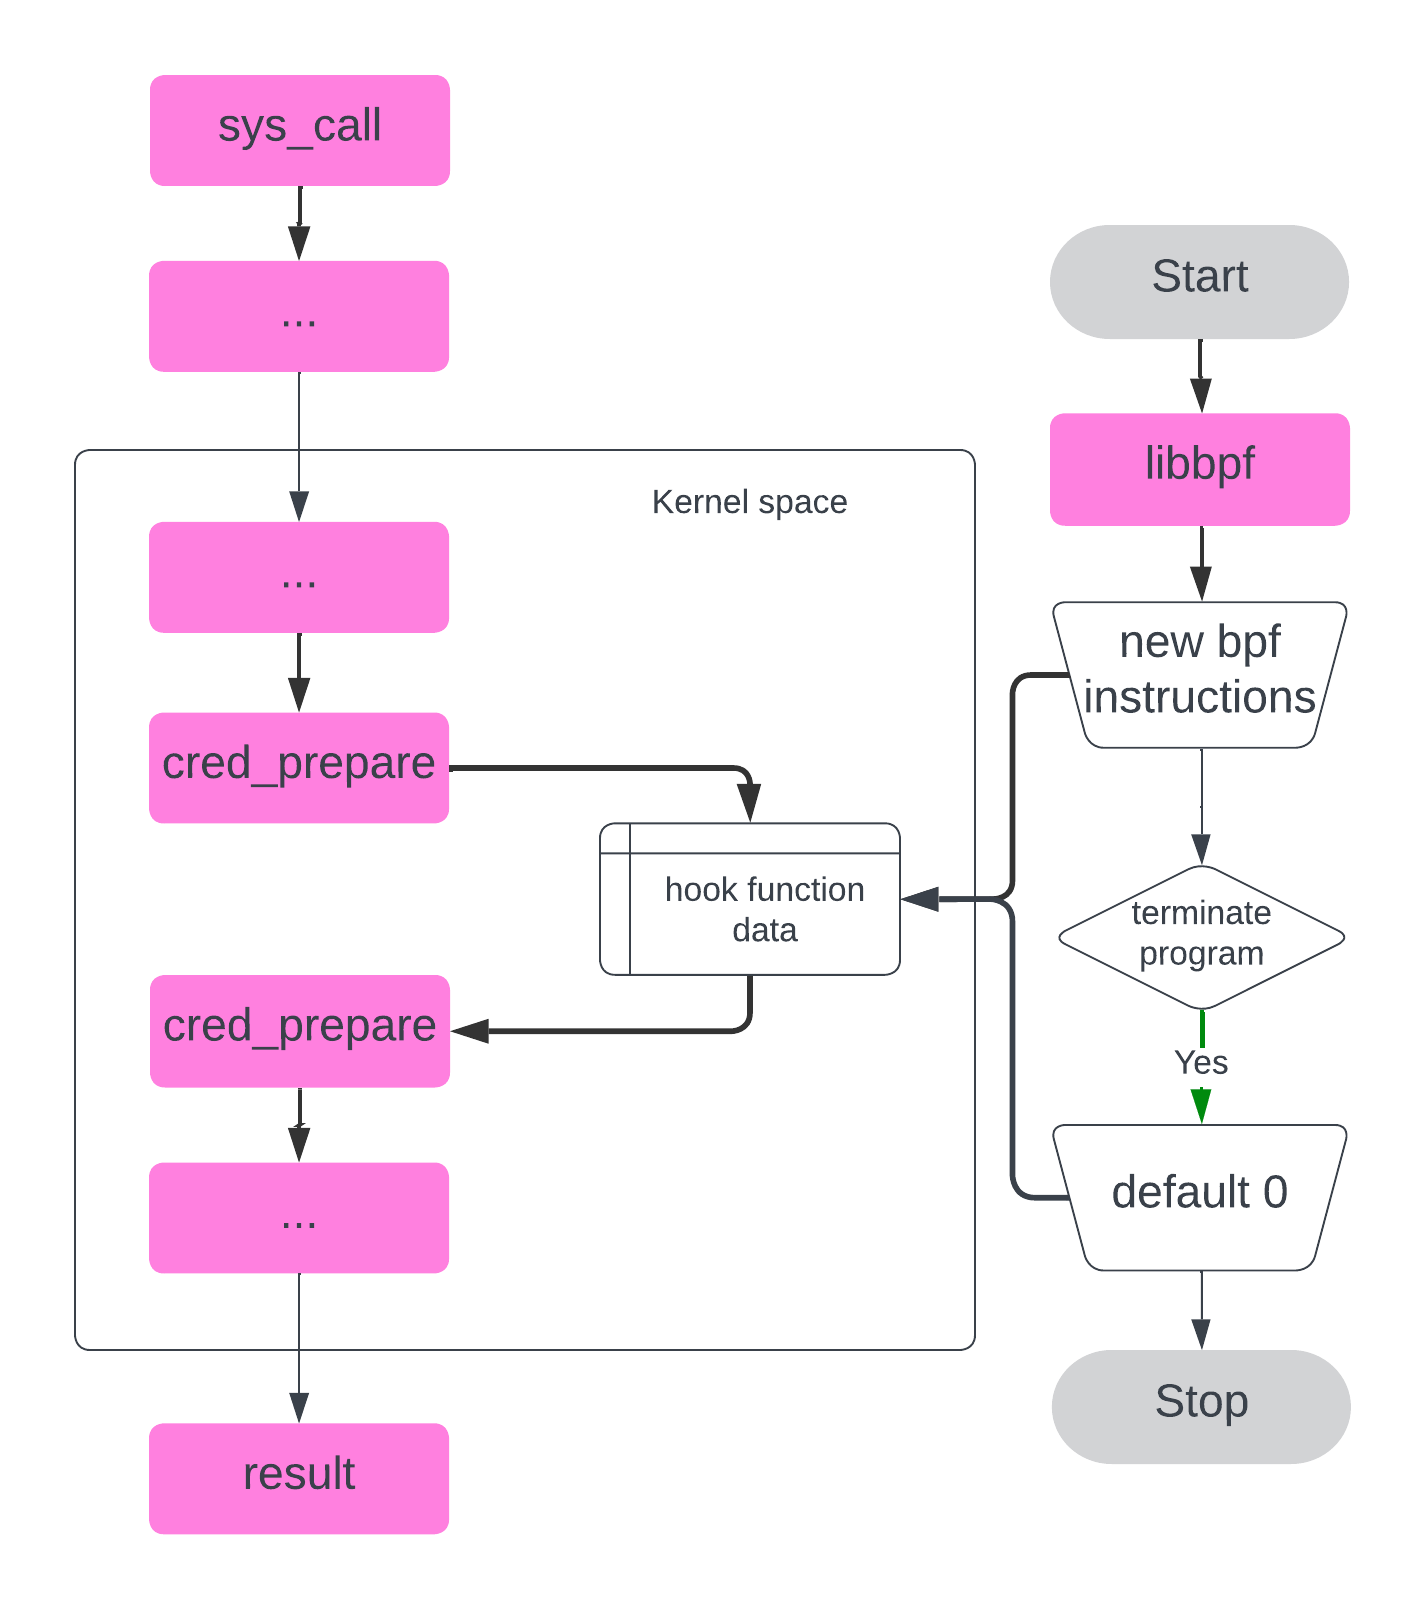
\includegraphics[width=\linewidth]{scheme.png}

\begin{flushleft}
	\ \\
	
	\ \\
	
	На данной схеме троеточием (...) обозначается незначительный процесс. Схема придерживается стандарта ГОСТ 19.701-90.
\end{flushleft}

\chapter{Определение хука}
\label{hook-0}

\begin{flushleft}
LSM (Linux Security Modules) предоставляет множество хуков, которые позволяют модулям безопасности внедрять свои политики и проверки в различные части ядра Linux. Эти хуки охватывают широкий спектр операций, таких как управление процессами, доступ к файловой системе, сетевые операции и другие.
	
Существует множество точек входа для внесения своего хука (\href{https://elixir.bootlin.com/linux/v6.1/source/security/selinux/hooks.c#L7116}{\underline{все selinux хуки}}). Но для нашей задачи выбран хук cred\_prepare:

Хук cred\_prepare вызывается при подготовке структуры учетных данных (credentials) для нового процесса. Это важный этап, потому что учетные данные включают в себя информацию о правах доступа и идентификацию процесса (например, идентификаторы пользователя и группы).

Благодаря этому хуку, мы можем отловить процесс исполнения интересующего системного вызова. Он может быть не только sys\_fchmod, но и, практически, любым другим (не для всех системных вызовов нужна структура учетных данных).
\end{flushleft}

\chapter{Работа программы}
\label{program}


\begin{flushleft}
	Теперь мы перейдем к описанию работы программы. Процесс может быть логически разделен на следующие ключевые компоненты:
	
	\begin{itemize}
		\item[1.] \textbf{Написание хука: } Это начальный этап, включающий разработку функции хука, которая будет интегрироваться в ядро для выполнения определенных задач безопасности.
		\item[2.] \textbf{Генерация низкоуровневых инструкций: } На этом этапе происходит трансляция кода хука в низкоуровневые инструкции, совместимые с внутренней архитектурой ядра.
		\item[3.] \textbf{Модификация сдвигов памяти для обращений к данным ядра: } Этот шаг включает корректировку смещений памяти при обращениях к данным ядра. В данном контексте следует ознакомиться с технологией Co-Re (Compile Once - Run Everywhere), реализованной в библиотеке libbpf, которая позволяет динамически адаптировать программы eBPF к разным версиям ядра.
		\item[4.] \textbf{Замена/регистрация нового хука: } После генерации и корректировки кода хука, производится его замена или регистрация в системе, что позволяет новому хуку получать данные ядра изнутри.
		\item[5.] \textbf{Безопасное отключение хука: } Обеспечение безопасного отключения хука, что включает его корректное удаление из системы и освобождение всех связанных ресурсов. Этот шаг важен для поддержания стабильности и безопасности системы.
	\end{itemize}
	
	Пункт 1 остается за нами. Пункты с 2 по 4 выполняются при помощи встроенных возможностей библиотеки libbpf, которая позволяет уменьшить объем работы в десятки раз. Пункт 5 является не столько задачей сделать что-то, сколько задачей не делать ничего: у bpf программ есть особенность внесения и изъятия - для их однократной отработки достаточно внести их в ядро с определенным триггером, но для постоянной нужны триггер (в нашем случае - это вызов хука) и дескриптор (это не совсем так, но для простоты объяснения оставлю) файла, в котором хранятся инструкции. В нашем случае, файлом являются данные работающей программы, что при её завершении автоматически удалятся, что приведет к изъятию bpf инструкций из ядра.
\end{flushleft}
\section{Работа программы. Main.}
\label{program-main}

\begin{flushleft}

\begin{verbatim}
    #include <bpf/libbpf.h>
    #include <unistd.h>
    #include "security.skel.h"
    
    int main(int argc, char *argv[])
    {
        struct security_bpf *skel;
        int err;
        skel = security_bpf__open_and_load();
        if (!skel) { 
            fprintf(stderr, "Ошибка генерации BPF каркаса.\n");
            goto cleanup;
        }
        err = security_bpf__attach(skel);
        if (err) {
            fprintf(stderr, "Ошибка внедрения BPF инструкций.\n");
            goto cleanup;
        }
        printf("BPF программа успешно загружена.\n");
        for (;;) {
            fprintf(stderr, ".");
            sleep(1);
        }
        cleanup:
        security_bpf__destroy(skel);
        return err;
    }
\end{verbatim}
    Структура security.c файла достаточно проста. Она использует возможности libbpf (в частности, утилиту bpftool) для генерации всего необходимого, в том числе и байт-инструкций. После чего этим же инструментом вносит программу в ядро и входит в бесконечный цикл.
\end{flushleft}
\section{Работа программы. BPF.}
\label{program-bpf}

\begin{flushleft}
    В случае с кодом хука всё интереснее: 
\begin{verbatim}
    #include <linux/bpf.h>
    #include <linux/capability.h>
    #include <linux/errno.h>
    #include <linux/sched.h>
    #include <linux/types.h>
    #include<linux/kernel.h>
    #include <bpf/bpf_tracing.h>
    #include <bpf/bpf_helpers.h>
    #include <bpf/bpf_core_read.h>
    
    #define X86_64_UNSHARE_SYSCALL 272
    #define UNSHARE_SYSCALL X86_64_UNSHARE_SYSCALL
    
    typedef unsigned int gfp_t;
    
    struct pt_regs {
        long unsigned int di;
        long unsigned int orig_ax;
    } __attribute__((preserve_access_index));
    
    typedef struct kernflagsel_cap_struct {
        __u32 cap[_LINUX_CAPABILITY_U32S_3];
    } __attribute__((preserve_access_index)) kernel_cap_t;
    
    struct cred {
        kernel_cap_t cap_permitted;
    } __attribute__((preserve_access_index));
    
    struct task_struct {
        unsigned int flags;
        const struct cred *cred;
    } __attribute__((preserve_access_index));
    
    char LICENSE[] SEC("license") = "GPL";
    SEC("lsm/cred_prepare")
    int BPF_PROG(handle_cred_prepare, struct cred *new, const struct cred *old, gfp_t gfp, int ret)
    {
        if (ret) return ret;
        
        struct pt_regs *regs;
        struct task_struct *task;
        int syscall;
        unsigned long flags;
        
        task = bpf_get_current_task_btf();
        regs = (struct pt_regs *) bpf_task_pt_regs(task);    
        syscall = regs -> orig_ax;
        
        if (syscall != UNSHARE_SYSCALL) return 0;
        
        flags = PT_REGS_PARM1_CORE(regs);
        if (!(flags & CLONE_NEWUSER)) {
            return 0;
        }
        
        return -EPERM;
    }
\end{verbatim}

Вдаваться в подробности каждой структуры не стану - это очень глубокая лужа, которая со стороны не кажется опасной. интереснее здесь \_\_attribute\_\_((preserve\_access\_index)) - макрос для компилятора и для дальнейшей релокации данных, который как раз магически определяет неоднозначное определение полей. Это относится к Co-Re технологии. В самом начале хука мы возвращаем ret - возвращенное значение предыдущего такого же хука. Это необходимо из-за того, что при внесении нашего хука, он добавляется в очередь на вызов хуков. То есть он может быть не единственным, из-за чего, для сохранения результата предыдущих хуков, все должны передавать результат дальше по списку (и да, на этом месте также можно реализовать вредоносную программу, которая попросту будет нарушать это, что приведет к неработоспособности других хуков безопасности). regs - регистры. Они хранят все внешние параметры для системного вызова. В целом, остальное всё понятно.

\end{flushleft}

\backmatter
\nocite{*}
\bibliographystyle{gost780u}
%s\bibliography{0-main}


\appendix   % Тут идут приложения


\end{document}
